\documentclass[border=4pt]{standalone}
\usepackage{tikz}
\usetikzlibrary{positioning, arrows.meta, shapes.geometric, calc, fit, backgrounds}
\usepackage{amsmath,amssymb}
\begin{document}
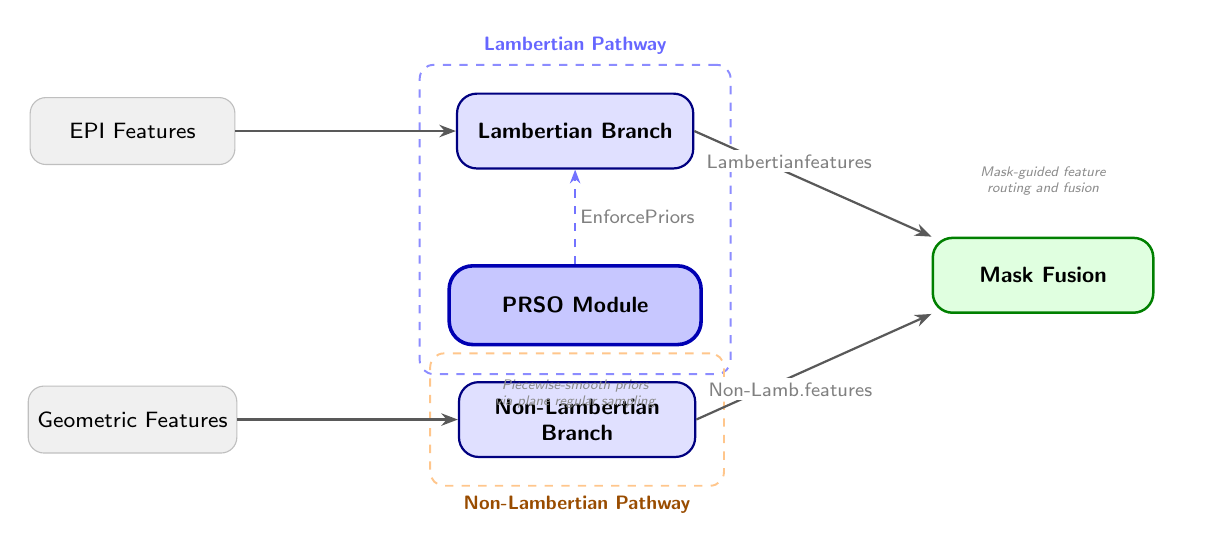
\begin{tikzpicture}[
  input/.style={draw, rounded corners=2mm, minimum width=2.6cm, minimum height=0.85cm,
                fill=gray!12, draw=gray!50, align=center,
                font=\sffamily\footnotesize},
  module/.style={draw, rounded corners=2.5mm, minimum width=3.0cm, minimum height=0.95cm,
                 fill=blue!12, draw=blue!50!black, line width=0.8pt, align=center,
                 font=\sffamily\footnotesize\bfseries},
  innov/.style={draw, rounded corners=3mm, minimum width=3.2cm, minimum height=1.0cm,
                fill=blue!22, draw=blue!70!black, line width=1.3pt, align=center,
                font=\sffamily\footnotesize\bfseries},
  output/.style={draw, rounded corners=2.5mm, minimum width=2.8cm, minimum height=0.95cm,
                 fill=green!12, draw=green!50!black, line width=0.9pt, align=center,
                 font=\sffamily\footnotesize\bfseries},
  arr/.style={-{Stealth[length=6pt]}, thick, color=black!65},
  arraux/.style={-{Stealth[length=5pt]}, thick, dashed, color=blue!55},
  lbl/.style={font=\sffamily\scriptsize, text=black!50, fill=white, inner sep=1.5pt},
  gbox/.style={draw=#1, dashed, rounded corners=5pt, inner sep=10pt, line width=0.7pt},
  annot/.style={font=\sffamily\tiny\itshape, text=black!45, align=center},
]

% ===== INPUT NODES (left column) =====
\node[input] (m1) {EPI Features};
\node[input, below=2.8cm of m1] (m2) {Geometric Features};

% ===== BRANCH NODES (center column) =====
\node[module, right=2.8cm of m1] (m3) {Lambertian Branch};
\node[module, right=2.8cm of m2] (m4) {Non-Lambertian\\Branch};

% ===== PRSO MODULE (innovation, below Lambertian Branch) =====
\node[innov, below=1.2cm of m3] (m5) {PRSO Module};

% ===== MASK FUSION (right column, centered vertically) =====
\node[output, right=3.0cm of $(m3.east)!0.5!(m4.east)$] (m6) {Mask Fusion};

% ===== MAIN FLOW ARROWS =====
% Inputs to branches
\draw[arr] (m1) -- (m3);
\draw[arr] (m2) -- (m4);

% Branches to fusion
\draw[arr] (m3.east) -- node[lbl, above, pos=0.4] {Lambertian\\[-1pt]features} (m6.north west);
\draw[arr] (m4.east) -- node[lbl, below, pos=0.4] {Non-Lamb.\\[-1pt]features} (m6.south west);

% PRSO to Lambertian Branch (innovation connection)
\draw[arraux] (m5) -- node[lbl, right, pos=0.5] {Enforce\\[-1pt]Priors} (m3);

% ===== GROUP BOXES (background layer) =====
\begin{scope}[on background layer]
  \node[gbox=blue!45, fit=(m3)(m5),
        label={[font=\sffamily\scriptsize\bfseries, text=blue!60]above:Lambertian Pathway}] (g1) {};
  \node[gbox=orange!45, fit=(m4),
        label={[font=\sffamily\scriptsize\bfseries, text=orange!60!black]below:Non-Lambertian Pathway}] (g2) {};
\end{scope}

% ===== KEY ANNOTATIONS =====
\node[annot, below=0.3cm of m5.south, text width=3.5cm]
  {Piecewise-smooth priors\\via plane regular sampling};
\node[annot, above=0.4cm of m6.north, text width=3.2cm]
  {Mask-guided feature\\routing and fusion};

\end{tikzpicture}
\end{document}